% Definizione del tipo di documento:
\documentclass[10pt, english, a4paper, titlepage, oneside]{book}

% Elenco package:
\usepackage[utf8]{inputenc}
\usepackage[top=2cm, left=1.5cm, bottom=2cm, right=1.5cm]{geometry}
\usepackage{titlesec}
\usepackage{graphicx,caption}
\usepackage{listings}
\usepackage{epstopdf}
\usepackage{float}
\usepackage{multirow}
\usepackage[dvipsnames,table]{xcolor}
\usepackage{amsmath}
\usepackage{multicol}
\usepackage{fancyhdr}
\usepackage{gensymb}
\usepackage{eurosym}
\usepackage{array}
\usepackage[acronym,nopostdot]{glossaries}
\newcolumntype{P}[1]{>{\centering\arraybackslash}p{#1}}
\newcolumntype{M}[1]{>{\centering\arraybackslash}m{#1}}

% Formato intestazione capitoli:
\titleformat{\chapter}
{\normalfont\Huge\filcenter\bf}
{}
{1pc}
{\MakeUppercase}
[\titlerule]
\fancypagestyle{plain}
{
  \fancyhf{}
  \fancyfoot[R]{\thepage}
  \renewcommand{\headrulewidth}{0pt}
  \renewcommand{\footrulewidth}{0pt}
}

% Posizione intestazione capitoli:
\titlespacing{\chapter}{0cm}{-1cm}{1.5cm}

% Formato intestazione pagina:
\pagestyle{fancy}
\fancyhead{}
\fancyhead[R]{\textbf{\MakeUppercase{\leftmark}}}
\fancyfoot{}
\fancyfoot[R]{\thepage}

% Lista acronimi
\makeglossaries
% use them with \acrshort{acronym_name} and \acrlong{acronym_name}
\newacronym{FPGA}{FPGA}{Field Programmable Gate Array}
\newacronym{MCU}{MCU}{MicroController Unit}
\newacronym{IP}{IP}{Intellectual Property}
\newacronym{RAM}{RAM}{Random Access Memory}
\newacronym{OCRAM}{OCRAM}{On-Chip Random Access Memory}
\newacronym{ROM}{ROM}{Read-Only Memory}
\newacronym{OCROM}{OCROM}{On-Chip Read-Only Memory}
\newacronym{SDR}{SDR}{Single Data Rate}
\newacronym{DDR}{DDR}{Double Data Rate}
\newacronym{FSM}{FSM}{Finite State Machine}
\newacronym{DUT}{DUT}{Device Under Test}
\newacronym{VCR}{VCR}{Virtual Configuration Register}
\newacronym{CR1}{CR1}{Configuration Register 1}
\newacronym{CR0}{CR0}{Configuration Register 0}


% CREAZIONE DOCUMENTO:
\begin{document} 

% Creazione titolo:
\begin{titlepage}
    \centerline{ \Huge\bf POLITECNICO DI TORINO }
    \vspace{2cm}
    \centerline{ \large Dipartimento di Elettronica e Telecomunicazioni } 
    \vspace{5mm}
    \centerline{ \large Corso di Laurea in Ingegneria Elettronica }
    \vspace{5mm}
    \centerline{ \large Tesi di Laurea Magistrale }
    \vspace{3cm}
    \centerline{ \includegraphics[width=4cm]{logopoli} }
    \vspace{3cm}
    \centerline{ \Huge\bf Design of FPGA IP for modular }
    \vspace{5mm}
    \centerline{ \Huge\bf architectures on VirtLAB board }
    \vspace{4cm}
    \centerline{ \large \textbf{Relatore}: prof. Massimo Ruo Roch }
    \vspace{5mm}
    \centerline{ \large \textbf{Laureando}: Andrea Bononi }
\end{titlepage}

\chapter*{ACKNOWLEDGEMENTS}

% Creazione indice:
\tableofcontents

% Creazione glossario:
\printglossary[type=\acronymtype, nonumberlist]

% -------------------------------------------------------------------------------------------------
\chapter{INTRODUCTION}
\noindent The recent SARS-CoV2 pandemic put a great strain on university courses. Despite the access to physical infrastructures was prohibited, videoconferencing and recorded videos allowed to proceed with the lectures without too many troubles. However, engineering teaching should also involve real laboratory experiences to provide students fundamental skills. When it comes to electronic lessons, it was usually not possible to provide the students the majority of the required instruments (such as digital oscilloscopes, signal generators and spectrum analyzers) given their high cost.  \\ \\ 
In this scenario, a low-cost experimental printed circuit board, namely the VirtLAB board, was developed at Politecnico di Torino to provide electronic students access to physical devices. Its architecture can be divided in two main sections \cite{virtlab}:
\vspace{2mm}
\begin{itemize}
    \item \textbf{User section}: it contains an \acrshort{MCU} (STM32L496) and an \acrshort{FPGA} (Intel Cyclone 10 LP), which can be easily programmed by the students for educational purposes, together with some LEDs and some switches.
    \vspace{1mm}
    \item \textbf{Master section}: it contains an MCU (STM32L496), an FPGA (Intel Cyclone 10 LP) and two external memories (a Hyper\acrshort{RAM} and a QSPI flash) to be used as generic data storage. From the point of view of a student, this side comes already programmed to provide a virtual replacement of the bench equipment.
\end{itemize} 
\vspace{3mm}
\begin{figure}[H]
    \centering
    \includegraphics[width=14cm]{virtlab_block_diagram.png}
    \vspace{5mm}
    \caption{VirtLAB board block diagram}
    \label{virtlab_block_diagram}
\end{figure}
\vspace{5mm}
Currently, it is still not possible to exploit the master section to its full potential. In particular, the FPGA might used to implement several useful applications it may realize. In this regard, the best approach would be to create modular architectures using generic \acrshort{IP} cores that share a common communication protocol, namely the Intel Avalon interface. In this way, it is possible to make full use of the features provided by the Intel CAD software:
\vspace{2mm}
\begin{itemize}
    \item Several general-purpose IP cores with an Intel Avalon interface are already provided by Intel, such as on-chip memories, processors and so on.
    \vspace{1mm}
    \item The Intel CAD software is able to automatically create the interconnection logic among \acrshort{IP} cores that use an Intel Avalon interface.
\end{itemize}
\vspace{4mm}
At the moment, it is not possible to create an Avalon-based modular architecture able to communicate with any of the external memory storage devices. Indeed, both the HyperRAM interface and the QSPI interface are quite different from the Intel Avalon interface. This paper deals with the design, developement and testing of a custom IP core able to convert the HyperRAM interface into an Intel Avalon interface, so that it can be easily managed by any modular architecture. The whole document refers to a HyperRAM model S27KL0641DA, i.e. the exact model employed in the VirtLAB board.
% -------------------------------------------------------------------------------------------------

% -------------------------------------------------------------------------------------------------
\chapter{SPECIFICATIONS} \label{specifications}
\section{Avalon Memory Mapped Interface}
\vspace{2mm}
The Avalon interface family defines different interfaces for different applications. What really matters for our purposes is the Avalon Memory Mapped interface, an address-based read/write interface typical of Host-Agent connections.
\vspace{6mm}
\begin{figure}[H]
    \centering
    \captionsetup{width=11.5cm}
    \includegraphics[width=12cm]{avalonMM_block_diagram.png}
    \vspace{2mm}
    \caption{\centering Typical Host-Agent system using components with an Avalon Memory Mapped interface (highlighted in light blue). The HyperRAM can be connected to the system only by using a suitable interface converter.}
    \label{avalonMM_block_diagram}
\end{figure}
\vspace{4mm}
\noindent The Avalon Memory Mapped interface includes some always-required signals and several optional signals that might be useful depending on the peripheral. In our case, some specific considerations have to be taken into account:
\vspace{2mm}
\begin{itemize}
    \item In general, the number of clock cycles required to read/write the HyperRAM is variable.
    \vspace{0.5mm}
    \item The system must support burst operations.
\end{itemize} 
\vspace{4mm}
Consequently, the Avalon Memory Mapped interface must include the following signals:
\vspace{2mm}
\begin{itemize}
    \item \textit{address}: the address to work with.
    \vspace{0.5mm}
    \item \textit{read}: it is asserted to indicate a read transfer.
    \vspace{0.5mm}
    \item \textit{write}: it is asserted to indicate a write transfer.
    \vspace{0.5mm}
    \item \textit{readdata}: the data read from the agent as a result of a a read transfer.
    \vspace{0.5mm}
    \item \textit{writedata}: the data to be written during a write transfer.
    \vspace{0.5mm}
    \item \textit{readdatavalid}: when asserted, it indicates that the readdata signal contains a valid data.
    \vspace{0.5mm}
    \item \textit{burstcount}: it indicates the number of transfers of a burst operation.
    \vspace{0.5mm}
    \item \textit{waitrequest}: it is asserted by the agent when it is unable to respond to a read/write request.
\end{itemize} 
\vspace{6mm}
\begin{figure}[H]
    \centering
    \includegraphics[width=17cm]{avalonMM_write_op.png}
    \vspace{5mm}
    \caption{Avalon Memory Mapped interface - write operation timing diagram}
    \label{avalonMM_write_op}
\end{figure}
\vspace{6mm}
\begin{figure}[H]
    \centering
    \includegraphics[width=17cm]{avalonMM_read_op.png}
    \vspace{5mm}
    \caption{Avalon Memory Mapped interface, read operation timing diagram}
    \label{avalonMM_read_op}
\end{figure}
\vspace{6mm}
\section{HyperRAM Interface Specifications} \label{HyperRAM Interface}
\vspace{2mm}
The HyperRAM interface is based on an 8-bit \acrshort{DDR} data bus used to transfer data, addresses and commands. The memory contains a couple of configuration registers that can be written in the same way as the memory locations, but using dedicated addresses. The interface includes the following signals:
\vspace{2mm}
\begin{itemize}
    \item \textit{CK}, \textit{CK}\# : differential clock.
    \vspace{1mm}
    \item \textit{RESET}\# : active-low hardware reset.
    \vspace{1mm}
    \item \textit{CS}\# : active-low chip select.
    \vspace{1mm}
    \item \textit{DQ}: 8-bit IO bus for data, addresses and commands.
    \vspace{1mm}
    \item \textit{RWDS}: read/write data strobe with the following functionality:
    \begin{itemize}
        \item During a read data transfer it is edge-aligned with DQ and it can be used to sample it.
        \item During a write data transfer it works as data masking signal.
        \item During a command transfer it indicates if additional latency is required.
    \end{itemize}
\end{itemize}
\vspace{6mm}
\begin{figure}[H]
    \centering
    \captionsetup{width=17cm}
    \includegraphics[width=18cm]{hram_read.png}
    \vspace{2mm}
    \caption{\centering HyperRAM interface, read operation timing diagram. During the data transfer, the memory drives both DQ and RWDS. During the command transfer, the host drives DQ and the memory drives RWDS: if RWDS is driven low, the access time is equal to $t_{acc}$ as shown, otherwise the access time is doubled.}
    \label{hram_read}
\end{figure}
\vspace{6mm}
\begin{figure}[H]
    \centering
    \captionsetup{width=17cm}
    \includegraphics[width=17.5cm]{hram_write.png}
    \vspace{2mm}
    \caption{\centering HyperRAM interface, write operation timing diagram. During the data transfer, the memory drives both DQ and RWDS. During the command transfer, the host drives DQ and the memory drives RWDS: if RWDS is driven low, the access time is equal to $t_{acc}$ as shown, otherwise the access time is doubled.}
    \label{hram_write}
\end{figure}
\vspace{6mm}
\begin{figure}[H]
    \centering
    \captionsetup{width=16.5cm}
    \includegraphics[width=15cm]{hram_write_reg.png}
    \vspace{2mm}
    \caption{\centering HyperRAM interface, register write operation timing diagram. DQ is always driven by the host.}
    \label{hram_write_reg}
\end{figure}
\begin{figure}[H]
    \centering
    \captionsetup{width=16.5cm}
    \includegraphics[width=17.5cm]{hram_timing_param.png}
    \vspace{2mm}
    \caption{\centering HyperRAM interface timing parameters.}
    \label{hram_timing_param}
\end{figure}
\vspace{4mm}
\subsection{Command-Address }
\vspace{2mm}
As we saw in section \ref{HyperRAM Interface}, the operation command and the addres are grouped in a 48-bit block, which is sent to the memory by the host one byte for clock level. Every bit of this block has its own meaning:
\vspace{4mm}
\begin{figure}[H]
    \centering
    \includegraphics[width=17.5cm]{CA.png}
    \vspace{3mm}
    \caption{Command-Address (CA) bit assignment}
    \label{CA}
\end{figure}
\vspace{1mm}
\subsection{Configuration Registers}
\vspace{2mm}
The S27KL0641DA HyperRAM contains two configuration registers that allow the user to set up different parameters.
\vspace{1mm}
\begin{figure}[H]
    \centering
    \includegraphics[width=16.5cm]{config_CA.png}
    \vspace{1mm}
    \caption{Command-Address configuration to access the configuration registers}
    \label{config_CA}
\end{figure}
\begin{figure}[H]
    \centering
    \includegraphics[width=16.5cm]{CR1.png}
    \vspace{1mm}
    \caption{Configuration Register 1 (\acrshort{CR1}) bit assignment}
    \label{CR1}
\end{figure}
\begin{figure}[H]
    \centering
    \includegraphics[width=16.5cm]{CR0.png}
    \vspace{1mm}
    \caption{Configuration Register 0 (\acrshort{CR0}) bit assignment}
    \label{CR0}
\end{figure}
\vspace{1mm}
\subsection{Deep Power Down Mode}
\vspace{2mm}
The HyperRAM can enter a special mode, called Deep Power Down (DPD) mode, in which the current consumption is driven to the lowest possible level. This mode is entered setting the \textit{Deep Power Down Enable} bit in CR0. The next access to the device, driving \textit{CS}\# low then high (dummy transaction), will cause the device to exit the DPD mode, as well as a hardware reset. A certain time is required to enter or exit the DPD mode.
\vspace{4mm}
\begin{figure}[H]
    \centering
    \includegraphics[width=15cm]{DPD_timing.png}
    \vspace{3mm}
    \caption{DPD timing diagram}
    \label{DPD_timing}
\end{figure}
\vspace{1mm}
\subsection{Power-Up}
\vspace{2mm}
The device must not be selected during the power-up, \textit{CS}\# has to remain high for a certain time. If \textit{RESET}\# is low during the power-up, the time counting does not start until \textit{RESET}\# goes high.
\vspace{4mm}
\begin{figure}[H]
    \centering
    \includegraphics[width=14cm]{powerup1.png}
    \vspace{3mm}
    \caption{Power-up with \textit{RESET}\# high}
    \label{powerup1}
\end{figure}
\vspace{2mm}
\begin{figure}[H]
    \centering
    \includegraphics[width=14cm]{powerup2.png}
    \vspace{3mm}
    \caption{Power-up with \textit{RESET}\# low}
    \label{powerup2}
\end{figure}
\section{Converter Design Specifications} \label{Converter Design Specifications}
\vspace{2mm}
Every HyperRAM interface uses a 32-bit addressing. However, the S27KL0641DA device is a 64 Mb memory partitioned in 16-bit words, therefore its addressing takes only 22 bits. On the other hand, the register space access requires dedicated addresses that are not in conflict with the ones related to the memory locations. \\ \\
In this design, it was decided to virtualize the memory access. To be more precise, the Avalon Memory Mapped interface refers to a 23-bit virtual address, that is translated by the interface converter in the corresponding physical address of the HyperRAM:
\vspace{2mm}
\begin{itemize}
    \item The virtual addresses from \textcolor{RoyalBlue}{0} to \textcolor{RoyalBlue}{$2^{22}-1$} correspond to the physical memory location addresses from \textcolor{RoyalBlue}{0} to \textcolor{RoyalBlue}{$2^{22}-1$}.
    \vspace{1mm}
    \item The virtual address \textcolor{RoyalBlue}{$2^{22}$} refers to a virtual configuration register that allows the user to set up different parameters. From the point of view of the Avalon interface, the host can only access the virtual configuration register, whereas the physical configuration registers of the HyperRAM cannot be accessed. In this way, it is possible to decide which parameters can be dynamically configured and which cannot.
    \vspace{1mm}
    \item The virtual addresses from \textcolor{RoyalBlue}{$2^{22} + 1$} to \textcolor{RoyalBlue}{$2^{23} - 1$} are reserved for future expansions.
\end{itemize}
\vspace{4mm}
The 16-bit virtual configuration register (\acrshort{VCR}) is organized in the following way:
\vspace{4mm}
\renewcommand{\arraystretch}{1.5}
\begin{table}[H]
    \begin{center}
        \begin{tabular}{|M{2cm}|M{5cm}|p{8cm}|}
            \hline
            \rowcolor{lightgray} VCR BIT & FUNCTION & \multicolumn{1}{|c|}{SETTINGS} \\
            \hline
            \multirow{2}{*}{0} & \multirow{2}{*}{Deep Power Down Enable} & 0: normal operation, exit DPD mode (default) \\
            & & 1: enter DPD mode \\
            \hline
            \multirow{2}{*}{1} & \multirow{2}{*}{Fixed Latency Enable} & 0: variable latency (default) \\
            & & 1: fixed latency \\
            \hline 
            2-15 & Reserved & Reserved for future expansions. \\
            \hline
        \end{tabular}
    \end{center}
\end{table}
\renewcommand{\arraystretch}{1}
\vspace{1mm}
\noindent By default, the memory works in normal mode. The host can force it to enter the DPD mode setting the \textit{Deep Power Down Enble} bit in VCR and then to go back to normal mode resetting that same bit. The interface converter shall detect any update of the \textit{Deep Power Down Enble} bit and consequently drive the memory according to figure \ref{DPD_timing}. Moreover, since a DPD exit request corresponds to a VCR update, it is possible for the host to update multiple parameters at the same time. For this reason, the interface converter must automatically drive a CR1 update after exiting the DPD mode. \\ \\
The default configuration of VCR does not match the default configuration of CR1 (figure \ref{CR1}). For this reason, the interface converter must automatically update CR1 after the power-up before allowing the host to start a new operation. \\ \\
As we can see from figures \ref{powerup1} and \ref{powerup2}, the interface converter must wait for the memory to power-up before allowing the host to start a new operation. Every time the memory is resetted, it must be powered-up again. \\ \\
\noindent As far as the frequency is concerned, the S27KL0641DA HyperRAM can work up to 100 MHz. However, the interface converter is designed to work at 50 MHz, sending to the memory a clock at that same frequency (as described in section \ref{Readdata Converter}).
% -------------------------------------------------------------------------------------------------

% -------------------------------------------------------------------------------------------------
\chapter{TEST ENVIRONMENT}
\noindent Before starting the interface converter design, it is necessary to define a test environment for it. We can exploit some of the IP cores provided by the CAD software (which are of course well-functioning) to create an Avalon Memory Mapped system suitable for the test. In particular, the test environment is an processor-based system that read some inputs and change the status of some LEDs according to it. The HyperRAM is employed as data memory for the processor.
\vspace{6mm}
\begin{figure}[H]
    \centering
    \includegraphics[width=12cm]{test_environment.png}
    \vspace{3mm}
    \caption{Test environment for the interface converter}
    \label{test_environment}
\end{figure}
\vspace{6mm}
\noindent To ensure that the test environment is well-functioning, the easiest way is to replace the DUT and the HyperRAM with an on-chip RAM, which can be obtained simply by using an IP core provided by the CAD software.
\vspace{6mm}
\begin{figure}[H]
    \centering
    \includegraphics[width=12cm]{test_environment_test.png}
    \vspace{3mm}
    \caption{Test environment verification}
    \label{test_environment_test}
\end{figure}
% -------------------------------------------------------------------------------------------------

% -------------------------------------------------------------------------------------------------
\chapter{DESIGN PARTITIONING}
% -------------------------------------------------------------------------------------------------
\noindent From now on, the interface converter is referred as \textit{avs\_hram\_converter}, i.e. the name of the custom IP implementing it. The top-level view of this IP is shown in figure \ref{toplevel}. On the Avalon side, the address line is on 23 bits and the data line is on 16 bits, as described in chapter \ref{specifications}, section \ref{Converter Design Specifications}. The burstcount signal is on 11 bits, i.e the maximum possible parallelism, corresponding to a theoretical maximum burst lenght equal to $2^{10}$ as stated in the Avalon documentation. 
\vspace{4mm}
\begin{figure}[H]
    \centering
    \includegraphics[width=6cm]{toplevel.png}
    \vspace{3mm}
    \caption{Top-level view of the interface converter}
    \label{toplevel}
\end{figure}
\vspace{4mm}
\noindent Unfortunately, it is usually not possible to push the burst lenght up to its theoretical maximum, since the duration of any memory operation is upper bounded. Considering that the latency of the converter depends on its implementation, it is not possible to estimate the actual upper bound of the burst lenght in advance. For this reason, the maximum parallelism is employed and the effective maximum of the burst lenght will be estimated after completing the design (section \ref{timing_constraints}).
\\ \\
\noindent The design follows a top-down approach. At first, it is important to point out the main features to be implemented:
\vspace{2mm}
\begin{itemize}
    \setlength\itemsep{2mm}
    \item \textbf{Command-Address building}: the Avalon input signals must be re-organized arranging the CA.
    \item \textbf{Configuration registers building}: every time the virtual configuration register is written, it is necessary to convert its content so that the physical configuration registers of the memory can be properly updated.
    \item \textbf{\acrshort{SDR} to \acrshort{DDR} conversion}: the 16-bit SDR data provided at the Avalon interface must be converted in an 8-bit DDR data to put it on the memory data bus.
    \item \textbf{DDR to SDR conversion}: the 8-bit DDR data provided by the memory (which is synchronous with RWDS and not with the internal clock) must be converted in a 16-bit SDR data and synchronized with the clock.
    \item \textbf{Clock shifting and clock gating}: the internal clock must by shifted by 90 degrees and properly gated before being sent to the memory.
    \item \textbf{Timer}: the system must be aware the passage of time to satisfy all the timing requirements.
    \item \textbf{Address reconstruction}. As we can see in figure \ref{avalonMM_write_op}, the host can interrupt a write operation at any time. However, the HyperRAM does not support this feature. For this reason, the interface converter must end the operation and start a new one when the burst is resumed. The new operation shall begin at the right address, i.e. the one immediately after the last written location. 
\end{itemize}
\vspace{4mm}
The CAD software provides an IP implementing a clock controller. Indeed, we can just create a custom IP implementing all the features except the clock gating (\textit{avs\_hram\_mainconv}) and combine it with the clock controller IP (\textit{clkctrl}) to create the interface converter (\textit{avs\_hram\_converter}), as shown in figure \ref{clkctrl}. The \textit{avs\_hram\_mainconv} IP is composed by an \acrshort{FSM}-based control unit (section \ref{CU}) and an execution unit (figure \ref{mainconv}):
\vspace{6mm}
\begin{figure}[H]
    \centering
    \captionsetup{width=15.5cm}
    \includegraphics[width=14.5cm]{clkctrl.png}
    \vspace{4mm}
    \caption{\centering Architecture of the \textit{avs\_hram\_converter} IP}
    \label{clkctrl}
\end{figure}
\vspace{1mm}
\begin{figure}[H]
    \centering
    \captionsetup{width=16cm}
    \includegraphics[width=18cm]{mainconv.png}
    \caption{\centering Execution unit of the \textit{avs\_hram\_mainconv} IP. Avalon signals are placed on the left. HyperRAM signals are placed on the right. The top green signals represent the control signals received from the control unit. The bottom red signals represent the status signals sent to the control unit.}
    \label{mainconv}
\end{figure}
\vspace{6mm}
\noindent The role of each block represented in figure \ref{mainconv} is described in the table below:
\vspace{4mm}
\renewcommand{\arraystretch}{1.5}
\begin{table}[H]
    \begin{center}
        \begin{tabular}{|p{3cm}|p{4cm}|p{3.5cm}|p{6cm}|}
            \hline
            \rowcolor{lightgray} \multicolumn{1}{|c|}{NAME} & \multicolumn{1}{|c|}{TYPE} & \multicolumn{1}{|c|}{NICKNAME} & \multicolumn{1}{|c|}{DESCRIPTION} \\
            \hline
            \textit{addr\_reg} & \textit{register} & address register & It stores the virtual address provided on the Avalon side. \\
            \hline
            \textit{datain\_reg} & \textit{register} & data register & It stores the input data provided on the Avalon side. \\
            \hline
            \textit{conf\_reg} & \textit{register} & configuration register & It implements the virtual configuration register as described in section \ref{Converter Design Specifications}. \\
            \hline
            \textit{burstcnt\_reg} & \textit{register} & burst lenght register & It stores the burst lenght value provided on the Avalon side. \\
            \hline
            \textit{CA\_builder\_inst} & \textit{CA\_builder} & CA builder & It builds the 48-bit Command-Address starting from the address value and the operation type. Refer to section \ref{CA Builder} for a detailed description. \\
            \hline
            \textit{CA\_unpacker\_inst} & \textit{CA\_unpacker} & CA unpacker & It separates the Command-Address in 3 different 16-bit data. Each of them can be picked out depending on the value of a selector. Refer to section \ref{CA Unpacker} for a detailed description. \\
            \hline
            \textit{conf\_builder\_inst} & \textit{conf\_builder} & configuration builder & It generates the content of the physical configuration registers of the HyperRAM starting from the content of the virtual configuration register. Refer to section \ref{Configuration Builder} for a detailed description. \\
            \hline
            \textit{writedata\_converter} & \textit{SDR\_to\_DDR\_converter} & writedata converter & It converts a 16-bit SDR data in a 8-bit DDR data, so that it can be channeled into the HyperRAM \textit{DQ} bus. Refer to section \ref{Writedata Converter} for a detailed description. \\
            \hline
            \textit{RWDS\_tracker} & \textit{dff} & RWDS tracker & It samples the value of RWDS using the internal clock. It is not suitable for sampling it while receiving a DDR data, it is intended to be used during the CA transmission. \\
            \hline
            \textit{dpdreq\_tracker} & \textit{dff} & DPD request tracker & It is employed to keep track of a DPD mode entry request. \\
            \hline
            \textit{op\_tracker} & \textit{dff} & operation tracker & It is employed to keep track of the type of operation currently in execution. \\
            \hline
            \textit{dpd\_tracker} & \textit{sr\_flipflop} & DPD tracker & It is employed to keep track of the current memory mode (NORMAL, DPD). \\
            \hline
            \textit{readdata\_converter} & \textit{DDR\_to\_SDR\_converter} & readdata converter & It samples \textit{RWDS} and \textit{DQ} using a 400 MHz clock, converting the 8-bit DDR data in a 16-bit SDR data. It also provides a version of RWDS with a rising-edge approximately center-aligned with the SDR data. Refer to section \ref{Readdata Converter} for a detailed description. \\
            \hline
            \textit{pll\_x8\_inst} & \textit{pll\_x8} & pll x8 & It generates a 400 MHz clock starting from the internal 50 MHz clock. \\
            \hline
            \rowcolor{lightgray} \multicolumn{4}{|c|}{CONTINUED...} \\
            \hline
        \end{tabular}
    \end{center}
\end{table}
\begin{table}[H]
    \begin{center}
        \begin{tabular}{|p{3cm}|p{4cm}|p{3.5cm}|p{6cm}|}
            \hline
            \rowcolor{lightgray} \multicolumn{1}{|c|}{NAME} & \multicolumn{1}{|c|}{TYPE} & \multicolumn{1}{|c|}{NICKNAME} & \multicolumn{1}{|c|}{DESCRIPTION} \\
            \hline
            \textit{synchronizer\_inst} & \textit{synchronizer} & synchronizer & It samples the 16-bit SRD at the output of readdata converter (using the center-aligned version of RWDS it provides) to synchronize it with the internal clock. It contains an 11-bit up-counter that can be accessed from outside. \\
            \hline
            \textit{burst\_detector} & \textit{comparator} & burst detector & It notifies the system when the burst lenght is greater than 1. \\
            \hline
            \textit{burst\_cmp} & \textit{comparator} & burst comparator & It is employed to notice when the burst transmission has reached its end (i.e. the burst lenght). \\
            \hline
            \textit{addressgen} & \textit{adder\_1pipe} & address generator & It is employed when a write burst operation is resumed (after being stopped) to generate the new starting address. \\
            \hline
            \textit{clk\_shifter} & \textit{ddl\_90} & clock shifter & It introduces a 90 degree delay on the internal clock. \\
            \hline
        \end{tabular}
    \end{center}
\end{table}
\renewcommand{\arraystretch}{1}
\vspace{2mm}
\section{Readdata Converter} \label{Readdata Converter}
\vspace{2mm}
As we can see in figure \ref{hram_read}, during the data transfer of a read operation the memory drives both \textit{DQ} and \textit{RWDS}, the former being edge-aligned to the latter. The effect of board traces can be neglected considering that the \textit{DQ} trace and the \textit{RWDS} trace have a similar lenght on the PCB. The main goal of \textit{readdata converter} is to introduce a proper delay on \textit{RWDS} so that it can be used to sample \textit{DQ}; in particular, referring to figure \ref{readdataconv}, \textit{DQ\_out} and \textit{RWDS\_out} shall be approximately center-aligned.
\vspace{6mm}
\begin{figure}[H]
    \centering
    \captionsetup{width=12cm}
    \includegraphics[width=9.5cm]{readdataconv.png}
    \vspace{2mm}
    \caption{\centering Top-level view of \textit{readdata converter}.}
    \label{readdataconv}
\end{figure}
\vspace{4mm}
\noindent Considering that \textit{RWDS} oscillates at the clock frequency, a first possibility would be to introduce a combinational delay. In this way, it would be possible to push the memory frequency up to 100 MHz (assuming that all the other blocks in the system are fast enough). Theoretically, the Intel Cyclone 10 LP FPGA allows to introduce a controlled combinational delay on its input pins; however, the documentation is really poor, especially when it comes to explaining how to do it in the CAD software. Due to the many troubles encountered, it was decided to follow a different approach. \\ \\
Instead of forcing a combinational delay, a very high frequency clock (oversampling clock) can be employed. In this way, \textit{RWDS} can be shifted using just a flip-flop chain. To do that, the system need first to oversample both \textit{RWDS} and \textit{DQ} to synchronize them with the high-frequency clock. During the oversampling, some samples are collected violating the setup-hold constraints and they must be considered invalid. Indeed, the oversampling frequency must be high enough to collect more valid samples than invalid samples within a semi-period of \textit{DQ} and \textit{RWDS}, even in the worst case scenario. \\ \\
To compute the minimum sampling frequency, a setup-hold time lower than 3/4 of the clock period has been considered (assumption that shall be verified during the synthesis). Considering a rising-edge sampling, in the worst case both the first and the last samples are not valid, therefore the oversampling frequency must be at least 10 times the memory frequency:
\vspace{4mm}
\begin{figure}[H]
    \centering
    \captionsetup{width=12cm}
    \includegraphics[width=17cm]{oversampling1.png}
    \vspace{2mm}
    \caption{\centering Oversampling frequency 10 times the memory frequency, single-edge sampling. The green samples are valid, the red samples are invalid.}
    \label{oversampling1}
\end{figure}
\vspace{4mm}
\noindent Switching to a double-edge sampling, in the worst case three samples are not valid, therefore the oversampling frequency must be at least 8 times the memory frequency:
\vspace{4mm}
\begin{figure}[H]
    \centering
    \captionsetup{width=13cm}
    \includegraphics[width=16cm]{oversampling2.png}
    \vspace{2mm}
    \caption{\centering Oversampling frequency 8 times the memory frequency, double-edge sampling. The green samples are valid, the red samples are invalid.}
    \label{oversampling2}
\end{figure}
\vspace{4mm}
\noindent The oversampling frequency is generated using a PLL available in the FPGA. As written in the Intel Cyclone 10 LP datasheet, the maximum output frequency of the PLL is equal to 472.5 MHz, therefore the memory frequency is upper bounded at 59 MHz (considering a double-edge sampling). In other words, to make the oversampling technique work it is not possible to push the memory frequency up to its maximum (100 MHz). Indeed, it was decided to lower the memory frequency to 50 MHz and to use a 400 MHz sampling frequency (generated by means of a PLL with a multiplication factor equal to 8). \\ \\
\noindent Another important parameter is the value of the shift to be introduced on \textit{RWDS}. Theoretically, it should be delayed by 1/4 of the clock period (5 ns, i.e. two sampling clock periods) to make it center-aligned with \textit{DQ}. However, in the real case the setup-hold violations must be taken into account. As we can see in figure \ref{oversampling3}, a delay of 5 ns may lead to an oscillation of \textit{RWDS\_out} too close to the next variation of \textit{DQ\_out}. Indeed, the goal of \textit{readdata converter} is to generate \textit{RWDS\_out} such that it can be used to sample \textit{DQ\_out} without introducing any setup-hold violation.
\vspace{6mm}
\begin{figure}[H]
    \centering
    \captionsetup{width=13cm}
    \includegraphics[width=18cm]{oversampling3.png}
    \caption{\centering Example of possible setup-hold violation during the oversampling. In this case, \textit{RWDS\_out} is shifted by two sampling clock cycles with respect to \textit{DQ\_out}.}
    \label{oversampling3}
\end{figure}
\vspace{4mm}
\noindent To make sure that no setup-hold violations are present, it is necessary to reduce the shift to a single sampling clock cycle (2.5 ns) as shown in figure \ref{oversampling4}.
\vspace{6mm}
\begin{figure}[H]
    \centering
    \captionsetup{width=16cm}
    \includegraphics[width=18cm]{oversampling4.png}
    \caption{\centering Timing digram with a single clock cycle shift between \textit{RWDS\_out} and \textit{DQ\_out}.}
    \label{oversampling4}
\end{figure}
\vspace{4mm}
\noindent As we already said, the goal of \textit{readdata converter} is to introduce a shift between \textit{RWDS\_out} and \textit{DQ\_out} so that the former can be employed to sample the latter. The sampling is implemented outside \textit{readdata converter} by means of a register having the clock pin connected to \textit{RWDS\_out} and the input data pin connected to \textit{DQ\_out} (referring to figure \ref{mainconv}, this register is located inside the \textit{synchronizer}). In this regard, it is important to highlight that the timing behavior described in figure \ref{oversampling4} works correctly only assuming that there are no other delay contributions between \textit{readdata converter} and the sampling register (i.e. that the delay between the clock pin and the input pin of the sampling register is exactly equal to the delay between \textit{DQ\_out} and \textit{RWDS\_out}). Unfortunately, this assumption cannot be considered true. In general, we must consider the circuit in figure \ref{oversampling5}.
\vspace{6mm}
\begin{figure}[H]
    \centering
    \captionsetup{width=18cm}
    \includegraphics[width=14cm]{oversampling5.png}
    \vspace{4mm}
    \caption{\centering Basic scheme of \textit{readdata converter}. All the delay terms are considered.}
    \label{oversampling5}
\end{figure}
\vspace{4mm}
\noindent To make \textit{readdata converter} work, it is necessary to estimate the value of the delay terms and compensate them. A basic timing analysis in which \textit{readdata converter} behaves as described in figure \ref{oversampling4} is reported in figure \ref{rwdsgen_undelayed}.
\vspace{4mm}
\begin{figure}[H]
    \centering
    \captionsetup{width=16cm}
    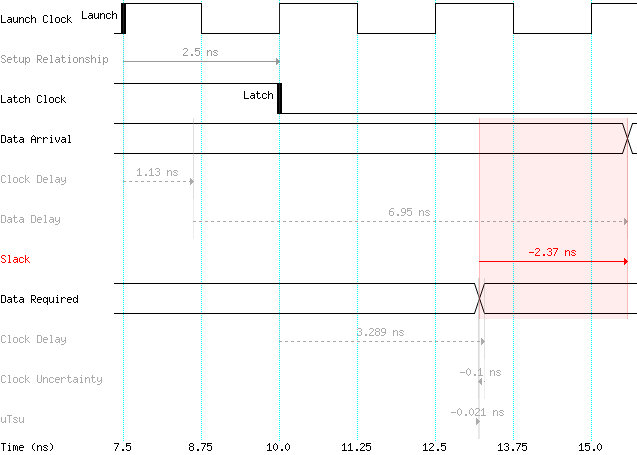
\includegraphics[width=16cm]{rwdsgen_undelayed.png}
    \vspace{4mm}
    \caption{\centering Timing analysis according to figure \ref{oversampling4}.}
    \label{rwdsgen_undelayed}
\end{figure}
\vspace{4mm}
\noindent As we can see in figure \ref{rwdsgen_undelayed}, \textit{RWDS\_out} (the latch clock) is delayed by 2.5 ns with respect to \textit{DQ\_out} as expected. However, the value of the input data pin of the sampling register (data arrival) changes 2.37 ns later than required (i.e. slightly less than a period of the high-frequency clock). To compensate this timing violation, \textit{readdata converter} can be designed to introduce a further shift of 2.5 ns (thus, a total delay of 5 ns), as shown in figure \ref{oversampling6}.
\vspace{6mm}
\begin{figure}[H]
    \centering
    \captionsetup{width=15cm}
    \includegraphics[width=17cm]{oversampling6.png}
    \vspace{2mm}
    \caption{\centering \textit{readdata converter} timing diagram able to prevent setup/hold violations.}
    \label{oversampling6}
\end{figure}
\vspace{4mm}
\noindent The timing diagram represented in figure \ref{oversampling6} is able to prevent setup/hold violation. However, it is not able to make the system in figure \ref{oversampling5} work. Indeed, \textit{RWDS\_out} cannot just shift \textit{RWDS\_oversampled}, since this signal may have spurious oscillations in correspondence of the invalid samples (which may assume whatever logic value). For this reason, the system oversamples \textit{RWDS\_in} and then implements a majority decision: when at least 5 samples out of 8 are different from the current decision about the value of \textit{RWDS\_in}, the current decision is toggled. Figure \ref{sampler_timing} represents some different scenarios, showing that the current decision does not display spurious oscillations regardless of the value assumed by the invalid samples. \textit{DDR\_in} is considered valid the clock period corresponding to the decision change; in this way, no setup/hold violations occour. \textit{RWDS\_out} is generated toggling a signal with 2 clock periods delay with respect to the variation of \textit{DDR\_out}, therefore setup/hold violations are prevented and no spurious oscillations are present. Moreover, its value is inverted with respect to the current decision, so that its rising edges correspond to the valid valued of \textit{SDR\_out}.
\vspace{6mm}
\begin{figure}[H]
    \centering
    \captionsetup{width=16cm}
    \includegraphics[width=18cm]{sampler_timing.png}
    \vspace{1mm}
    \caption{\centering Timing diagram of different scenarios during the oversampling. Three samples per \textit{RWDS\_in} period are not valid (worst-case). The values of \textit{RWDS\_oversampled} highlighted in red are invalid (they corresponds to a setup/hold violation, therefore they may assume whatever logic value). The values of \textit{RWDS\_oversampled} highlighted in green are valid. The current decision is obtained through a combinational circuit and it is sampled by the rising edge of the high-frequency clock.}
    \label{sampler_timing}
\end{figure}
\vspace{4mm}
\noindent The architecture of \textit{readdata converter} implementing the timing diagram in figure \ref{sampler_timing} is divided in an execution unit (described in subsection \ref{readdataconv_EU}) and a control unit (described in subsection \ref{readdataconv_CU}) implemented as a finite-state machine. As we can see in figure \ref{DDR_to_SDR_converter_EU}, the execution unit is strongly pipelined to be able to work with a 400 MHz clock frequency. Indeed, the circuit generating the current decision from the collected samples is not combinational, differently from what is assumed in figure \ref{sampler_timing}, and the control signals generated by the control unit are pipelined too. Consequently, the actual timing diagram is slightly different from the one shown in figure \ref{sampler_timing}, since a certain latency is introduced. However, the working principle remains the same.
\vspace{6mm}
\subsection{Execution Unit} \label{readdataconv_EU}
\vspace{2mm}
\noindent Figure \ref{DDR_to_SDR_converter_EU} represents the architecture of the execution unit of \textit{readdata converter}. The current decision about the value of \textit{RWDS\_in} is stored in a dedicated type-T flip-flop, namely the \textit{tracker}. Two different flip-flop chains are used to oversample \textit{RWDS\_in} on both rising and falling edges of the high-frequency clock. The majority decision is implemented using a \textit{voter} and some logic gates. In particular, the \textit{voter} is able to notice if the sum of all the collected samples is equal (\textit{eq4}) or greater (\textit{gt4}) than four. If the sum is greater than four (which means that there are more samples equal to logic 1 than to logic 0) and the current decision (stored in the \textit{tracker}) is logic 0, the decision is toggled. If the sum is lower than four (neither \textit{eq4} nor \textit{gt4} are set, thus there are more samples equal to logic 0 than to logic 1) and the current decision is logic 1, the decision is toggled.
\vspace{2mm}
\begin{figure}[H]
    \centering
    \captionsetup{width=16cm}
    \includegraphics[width=18cm]{DDR_to_SDR_converter_EU.png}
    \caption{\centering Execution unit of \textit{readdata converter}. The top green signals are the control signals received from the control unit, whereas the bottom red signals are the status signals sent to the control unit.}
    \label{DDR_to_SDR_converter_EU}
\end{figure}
\vspace{4mm}
\subsection{Voter}
\vspace{2mm}
The \textit{voter} is able to compute the sum of its inputs and to notice if the result is equal (\textit{eq4}) or greater (\textit{gt4}) than four. As we can see in figure \ref{voter}, it is diveded in five different pipeline stages. The sum is computed by means of a set of half-adders and full-adders. Starting from the sum, \textit{eq4} and \textit{gt4} are generated using some logic gates.
\vspace{6mm}
\begin{figure}[H]
    \centering
    \captionsetup{width=10cm}
    \includegraphics[width=15cm]{voter.png}
    \vspace{4mm}
    \caption{\centering Architecture of the \textit{voter}.}
    \label{voter}
\end{figure}
\vspace{2mm}
\subsection{Control Unit} \label{readdataconv_CU}
\vspace{2mm}
\begin{figure}[H]
    \centering
    \captionsetup{width=15cm}
    \includegraphics[width=11cm]{DDR_to_SDR_converter_CU.png}
    \vspace{4mm}
    \caption{\centering Control unit of \textit{readdata converter}. It lets the data pass through the \textit{lsb} register or the \textit{msb} when a variation of decision is detected (refer to figure \ref{readdataconv_EU} for the execution unit). The register (\textit{msb} or \textit{lsb}) are selected alternatively to reconstruct a 16-bit SDR data.}
    \label{DDR_to_SDR_converter_CU}
\end{figure}
\vspace{6mm}
\section{Synchronizer} \label{Synchronizer}
\vspace{2mm}
As described in section \ref{Readdata Converter}, \textit{readdata converter} generates a 16-bit SDR output and a properly shifted strobe to sample it. The SDR output can be connected to the input data pin of a sampling register having the clock pin connected to the strobe, as shown in figure \ref{oversampling5}. However, in this way the data is not synchronized to the 50 MHz clock. \\ \\
The main goal of the \textit{synchronizer}, apart from providing the sampling register, is to synchronize the data with the 50 MHz clock. The main idea is to alternate multiple sampling registers, so that the sampled data remains available for a longer time. The architecture is divided in an execution unit (figure \ref{synchronizer_EU}) and a control unit (figure \ref{synchronizer_CU}).
\vspace{4mm}
\begin{figure}[H]
    \centering
    \captionsetup{width=10cm}
    \includegraphics[width=6cm]{synchronizer_toplevel.png}
    \vspace{2mm}
    \caption{\centering Top-level view of the \textit{synchronizer}.}
    \label{synchronizer_toplevel}
\end{figure}
\vspace{2mm}
\begin{figure}[H]
    \centering
    \captionsetup{width=10cm}
    \includegraphics[width=18cm]{synchronizer.png}
    \caption{\centering Execution unit of the \textit{synchronizer}.}
    \label{synchronizer_EU}
\end{figure}
\vspace{4mm}
\noindent The actual synchronization is implemented by means of a set-reset flip-flop, namely the \textit{synch\_flipflop}, having the clock pin connected to the strobe, the set pin always set to logic 1 (assuming that the system is enabled) and the output pin connected to the FSM as a status signal called \textit{start\_sampling}. The strobe is asynchronous to the clock, therefore a variation of \textit{start\_sampling} may lead to setup/hold violations; in other words, the control unit may take more than one clock cycle to detect a variation of \textit{start\_sampling}. However, since the sampled data is available for multiple clock cycles, this does not represent a problem. The timing diagram in figure \ref{synch_timing} refers to a condition in which the activation of \textit{start\_sampling} is detected with a delay of 1 clock cycle.
\vspace{6mm}
\begin{figure}[H]
    \centering
    \captionsetup{width=10cm}
    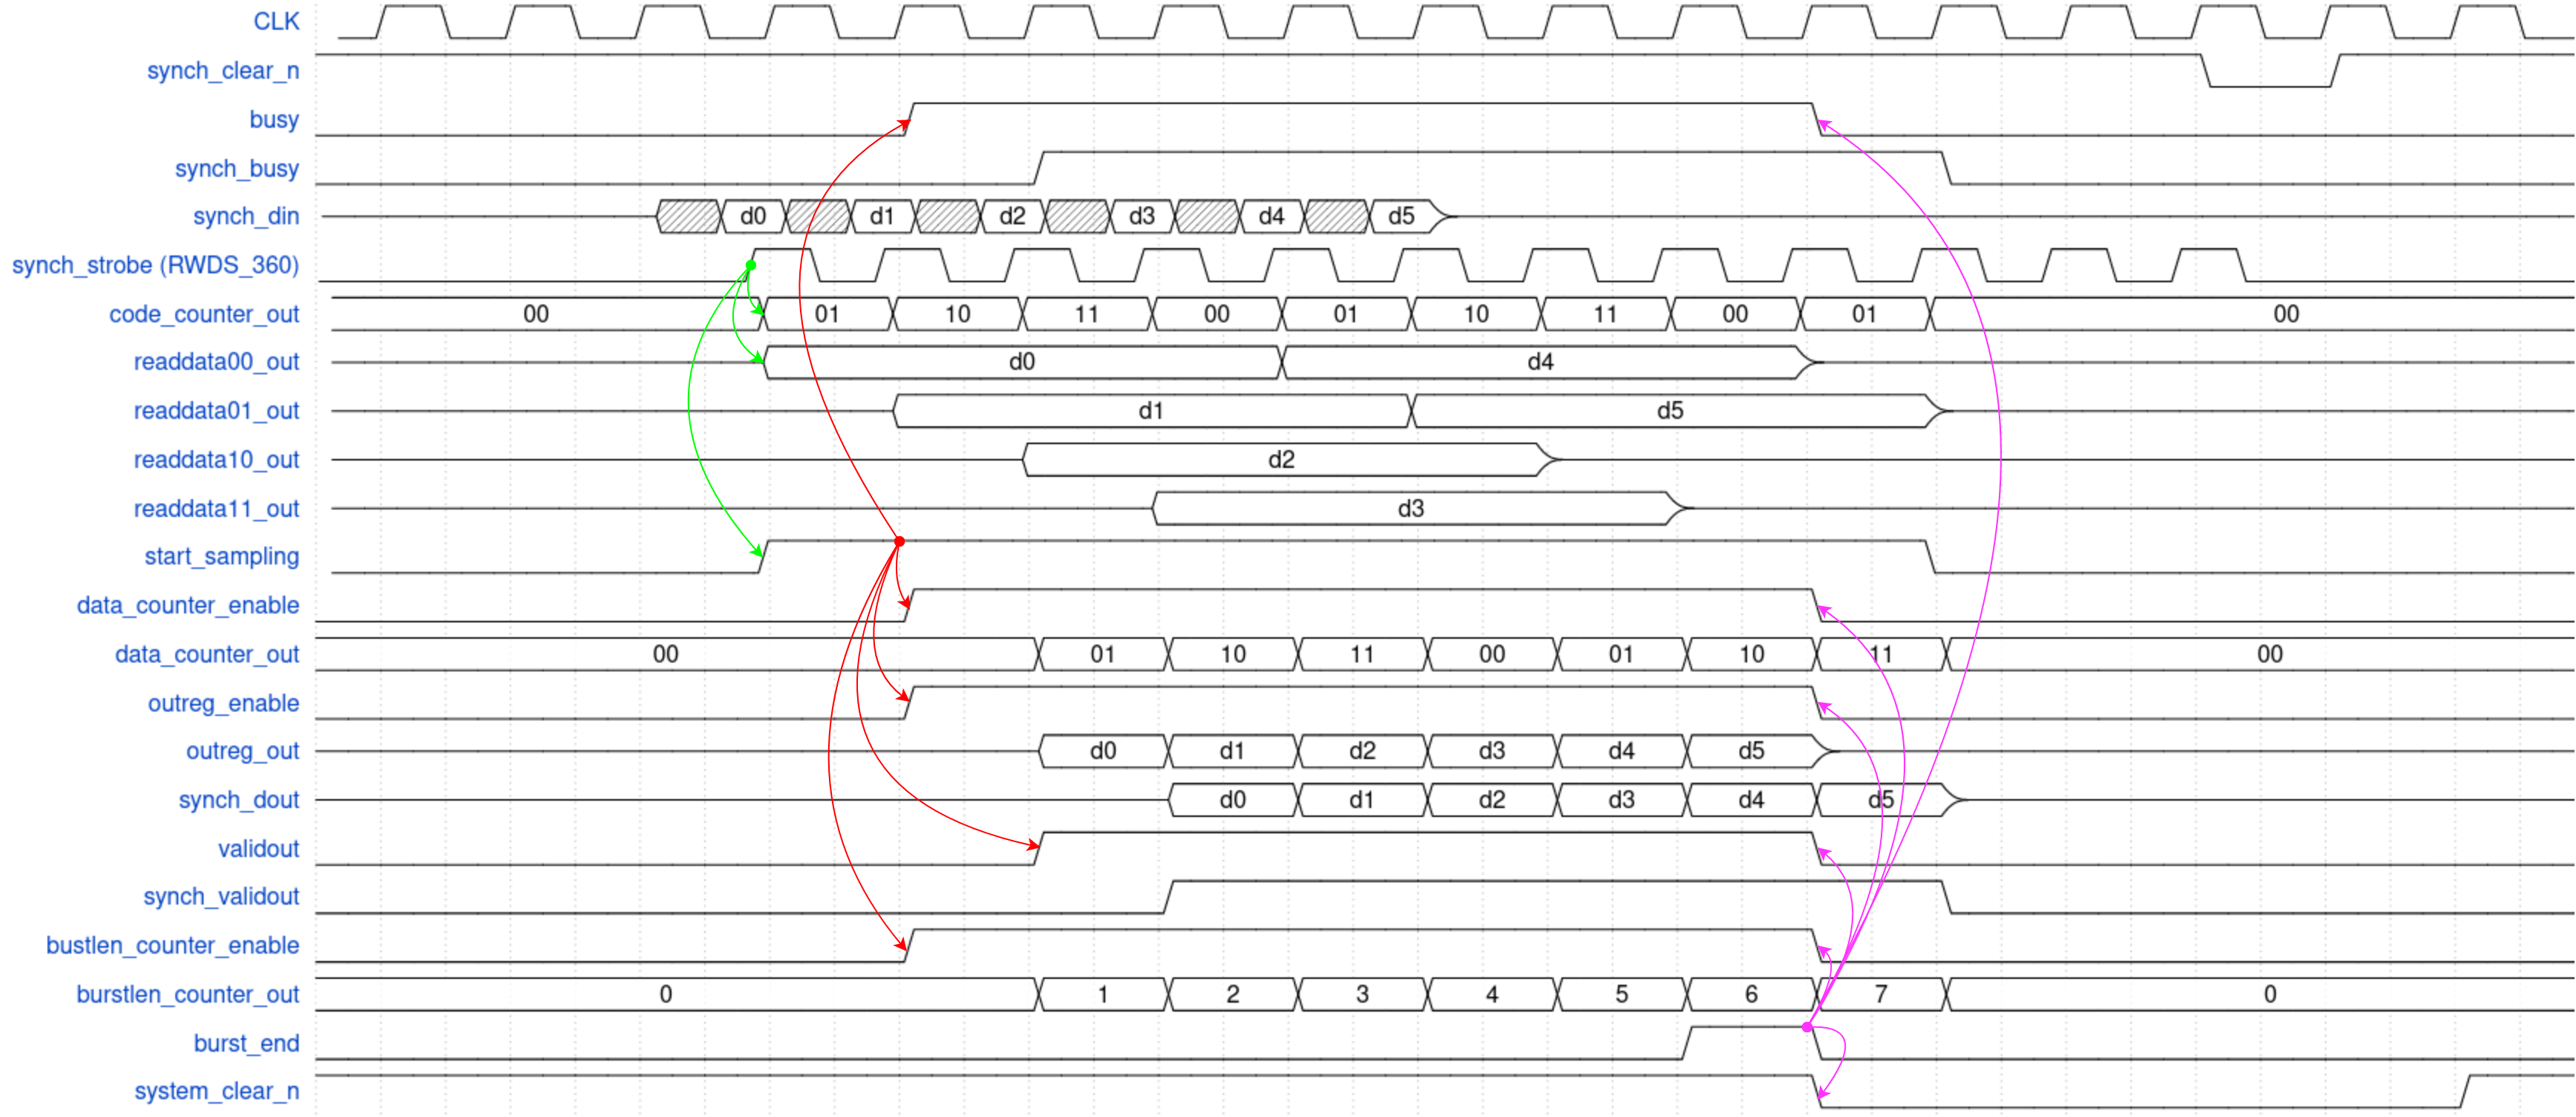
\includegraphics[width=18cm]{synch_timing.png}
    \caption{\centering Timing diagram of the \textit{synchronizer}.}
    \label{synch_timing}
\end{figure}
\vspace{4mm}
\begin{figure}[H]
    \centering
    \captionsetup{width=14cm}
    \includegraphics[width=10cm]{synchronizer_CU.png}
    \vspace{4mm}
    \caption{\centering Control unit (finite-state machine) of the \textit{synchronizer}.}
    \label{synchronizer_CU}
\end{figure}
\vspace{4mm}
\noindent The \textit{synchronizer} is able to notice when the burst to be transferred is completed. The burst lenght is stored in a dedicated register called \textit{burstlen}. The counter employed to keep track of the burst progress, namely the \textit{burstlen\_counter}, is made available outside, so that it can be employed independently when the \textit{synchronizer} is not enabled. \\ \\
Once the burst transfer is completed, the \textit{synchronizer} remains in a state in which the FSM constantly reset all the components by means of the \textit{system\_clear\_n} control signal, therefore it is not able to receive a new data burst. The activation of \textit{system\_clear\_n} may be detected with a certain delay by the componend that are clocked by the strobe, since it is synchronous to the clock. However, \textit{system\_clear\_n} remains active for many clock cycles, therefore this does not represent a problem. To restart the \textit{synchronizer} and make it able to reveive a new burst, it is necessary to manually set the \textit{synch\_clear\_n} signal after detecting \textit{synch\_busy} low, as shown in figure \ref{synch_timing}. \\ \\
The \textit{synchronizer} comes with an enable signal, namely \textit{synch\_enable}. As we can see in figure \ref{synchronizer_CU}, this signal must be set before beginning a burst transfer (i.e. before the strobe starts oscillating), otherwise the strobe edges are ignored. Setting \textit{synch\_enable} after beginning a burst transfer causes an unknowk behavior. If \textit{synch\_enable} is deactivated before completing a burst trasfer, the transfer is completed anyway.
\vspace{6mm}
\section{CA Builder} \label{CA Builder}
\vspace{2mm}
The 48-bit Command-Address is generated rearranging the bits of the address and combining them with the information about the operation type, as shown in figure \ref{CA_builder}.
\vspace{6mm}
\begin{figure}[H]
    \centering
    \captionsetup{width=14cm}
    \includegraphics[width=14cm]{CA_builder.png}
    \vspace{4mm}
    \caption{\centering Architecture of the \textit{CA builder}.}
    \label{CA_builder}
\end{figure}
\vspace{4mm}
\section{Writedata Converter} \label{Writedata Converter}
\vspace{2mm}
The Avalon side of the system works with a 16-bit SDR data, which must be converted in a 8-bit DDR data to be channeled in the HyperRAM DQ bus. This conversion is implemented in the \textit{writedata converter}. A multiplexer having the selector connected to the system clock is exploited to alternate the more-significant byte and the less-significant byte of the SDR data, as represented in figure \ref{writedata_converter}.
\vspace{6mm}
\begin{figure}[H]
    \centering
    \captionsetup{width=16cm}
    \includegraphics[width=16cm]{writedata_converter.png}
    \vspace{4mm}
    \caption{\centering Top view (on the left) and internal architecture (on the right) of the \textit{writedata converter}.}
    \label{writedata_converter}
\end{figure}
\vspace{2mm}
\section{Configuration Builder} \label{Configuration Builder}
\vspace{2mm}
From the Avalon side, the host can only refer to the virtual configuration register. However, every time the virtual configuration register is written, the content of the physical configuration registers of the memory shall be updated. The \textit{configuration builder} generates the content of the physical configuration registers starting from the content of the virtual configuration register, as shown in figure \ref{conf_builder}.
\vspace{6mm}
\begin{figure}[H]
    \centering
    \captionsetup{width=14cm}
    \includegraphics[width=12cm]{conf_builder.png}
    \vspace{4mm}
    \caption{\centering Architecture of the \textit{configuration builder}.}
    \label{conf_builder}
\end{figure}
\vspace{4mm}
\section{CA Unpacker} \label{CA Unpacker}
\vspace{2mm}
The 48-bit Command-Address generated by the \textit{CA builder} must be separated in three different 16-bit segments (namely \textit{CA0}, \textit{CA1} and \textit{CA2}), so that it can be fed to the \textit{writedata converter} and channeled in the HyperRAM DQ bus. This separation is implemented by the \textit{CA unpacker}, represented in figure \ref{CA_unpacker}. The selection between \textit{CA0}, \textit{CA1} and \textit{CA2} is achieved through a dedicated selector.
\vspace{6mm}
\begin{figure}[H]
    \centering
    \captionsetup{width=16cm}
    \includegraphics[width=16.5cm]{CA_unpacker.png}
    \vspace{4mm}
    \caption{\centering Top view (on the left) and internal architecture (on the right) of the \textit{CA unpacker}.}
    \label{CA_unpacker}
\end{figure}
\vspace{4mm}
\section{Address Generator} \label{Address Generator}
\vspace{2mm}
When it comes to the Avalon communication protocol, the host can interrupt the burst transfer at any time during a write operation. However, the HyperRAM protocol does not support this feature. For this reason, the interface converter must terminate the operation toward the HyperRAM when the host interrupts the transfer and begin a new operation when the transfer is resumed. Consequently, any interruption of the transfer implies to reconstruct the start address (i.e. the address from which to start the operation) and to send again the command-address to the memory. For this reason, a burst interruption is really expensive in terms of latency and it would be better to avoid it. \\ \\
During a write operation, the burst progress is tracked by means of the 11-bit counter provided by the \textit{synchronizer} (\textit{burstlen counter} referring to figure \ref{synchronizer_EU}). When the host interrupts and resumes the transfer, the new start address can be generated from the output of this counter. In this regard, it is important to make some considerations:
\begin{itemize}
\vspace{2mm}
    \item During a burst transfer the counter output is always two steps ahead with respect to the actual burst progress, so that the control unit can detect in advance when the burst is about to terminate (figure \ref{mainconv_CU}).
    \vspace{1mm}
    \item When a burst transfer is interrupted (i.e. when the control unit switches from the \textit{WRITEBURST} status to the \textit{STOP\_BURST\_1} status) the counter out increases by one more step, although a new data has not been transferred (figure \ref{mainconv_CU}).
    \vspace{1mm}
    \item The initial address provided by the host (namely the base address) remains stored in \textit{addr\_reg} (figure \ref{mainconv}) until the trasfer is completed.
\end{itemize}
\vspace{3mm}
All this considered, the start address can be reconstructed as \textit{new start address} = \textit{base address} + \textit{counter out} - 3. Three pipeline registers are placed on the counter output (\textit{cntpipe1}, \textit{cntpipe2} and \textit{cntpipe3} in figure \ref{mainconv}) to obtain \textit{counter out} - 3, whereas the sum with the base address is implemented using an adder (\textit{addressgen} in figure \ref{mainconv}).
\vspace{6mm}
\section{Control Unit and Timing Diagrams} \label{CU}
\begin{figure}[H]
    \centering
    \captionsetup{width=14cm}
    \includegraphics[width=18cm]{mainconv_CU.png}
    \caption{\centering Control unit of the \textit{avs\_hram\_mainconv} IP. Turquoise block: reset and power-on process. Grey block: DPD mode exit process. Green block: configuration registers update. Purple block: read operation. Blue block: write operation.}
    \label{mainconv_CU}
\end{figure}
\vspace{4mm}
\begin{figure}[H]
    \centering
    \captionsetup{width=11cm}
    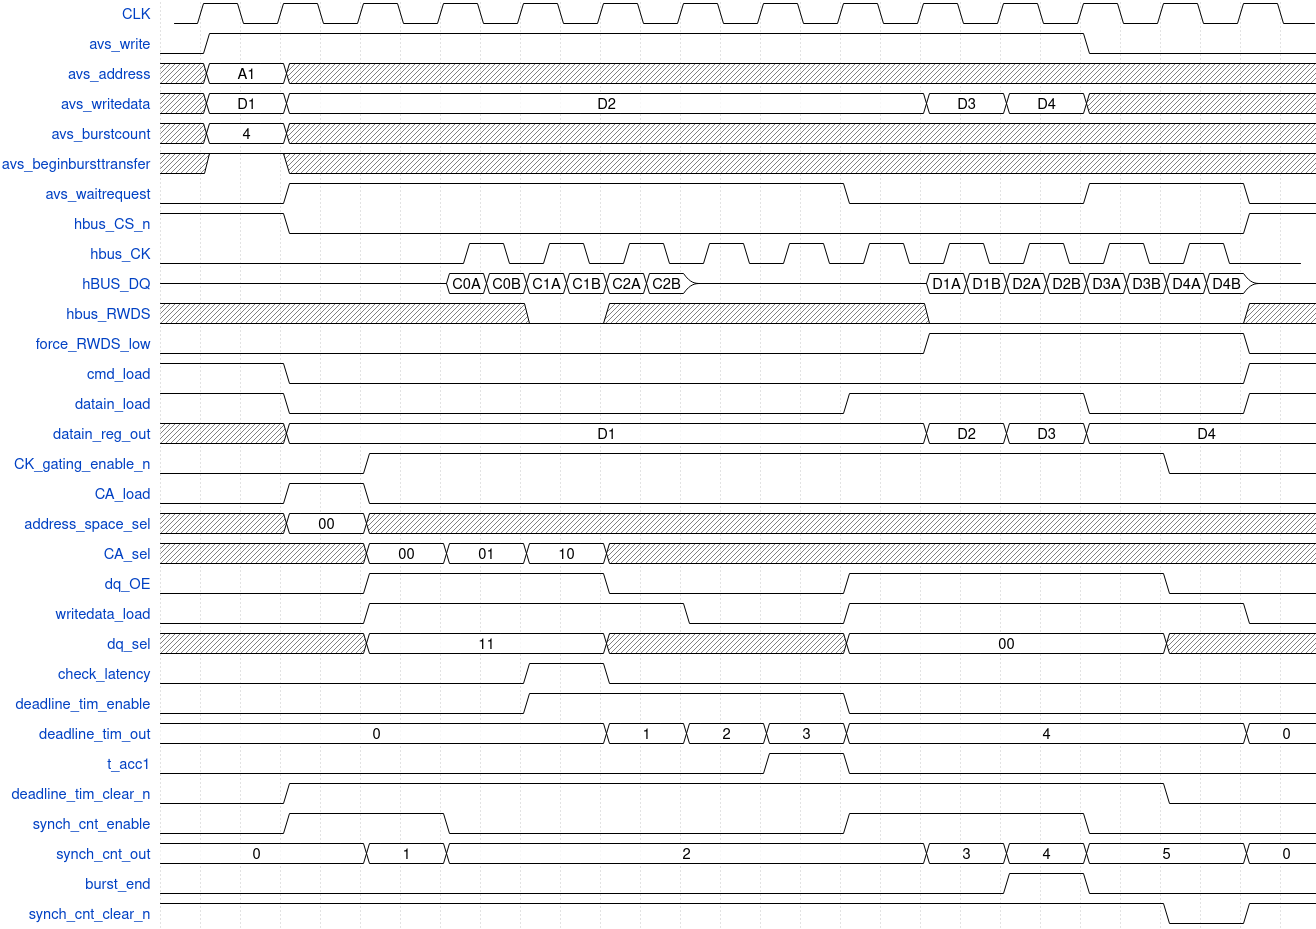
\includegraphics[width=18cm]{conv_writeburst_nostop.png}
    \caption{\centering Write burst operation. The Avalon signals vary according to figure \ref{avalonMM_write_op}. The HyperRAM signals match the timing in figure \ref{hram_write}.}
    \label{conv_writeburst_nostop}
\end{figure}
\begin{figure}[H]
    \centering
    \captionsetup{width=13cm}
    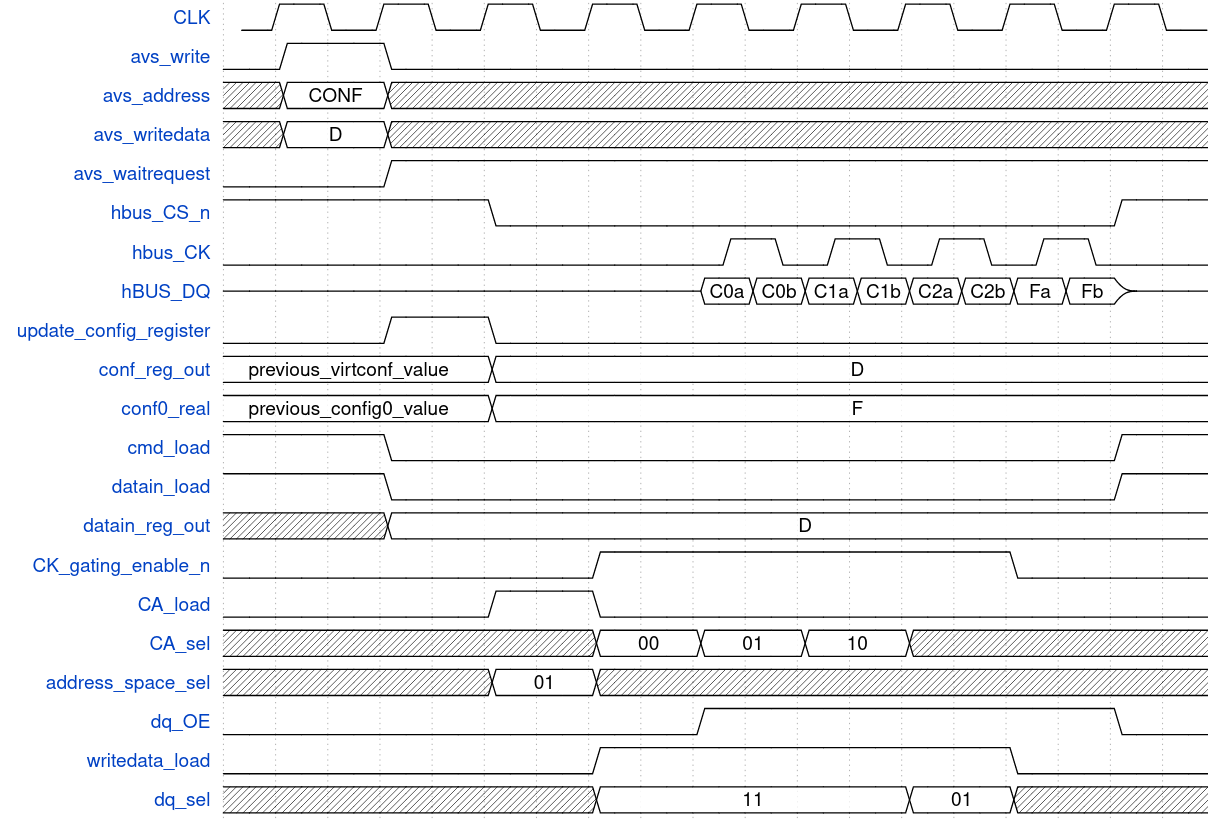
\includegraphics[width=13cm]{conv_writeconfig.png}
    \caption{\centering Configuration register update operation. The Avalon signals vary according to figure \ref{avalonMM_write_op}. The HyperRAM signals match the timing in figure \ref{hram_write_reg}.}
    \label{conv_writeconfig}
\end{figure}
\begin{figure}[H]
    \centering
    \captionsetup{width=16cm}
    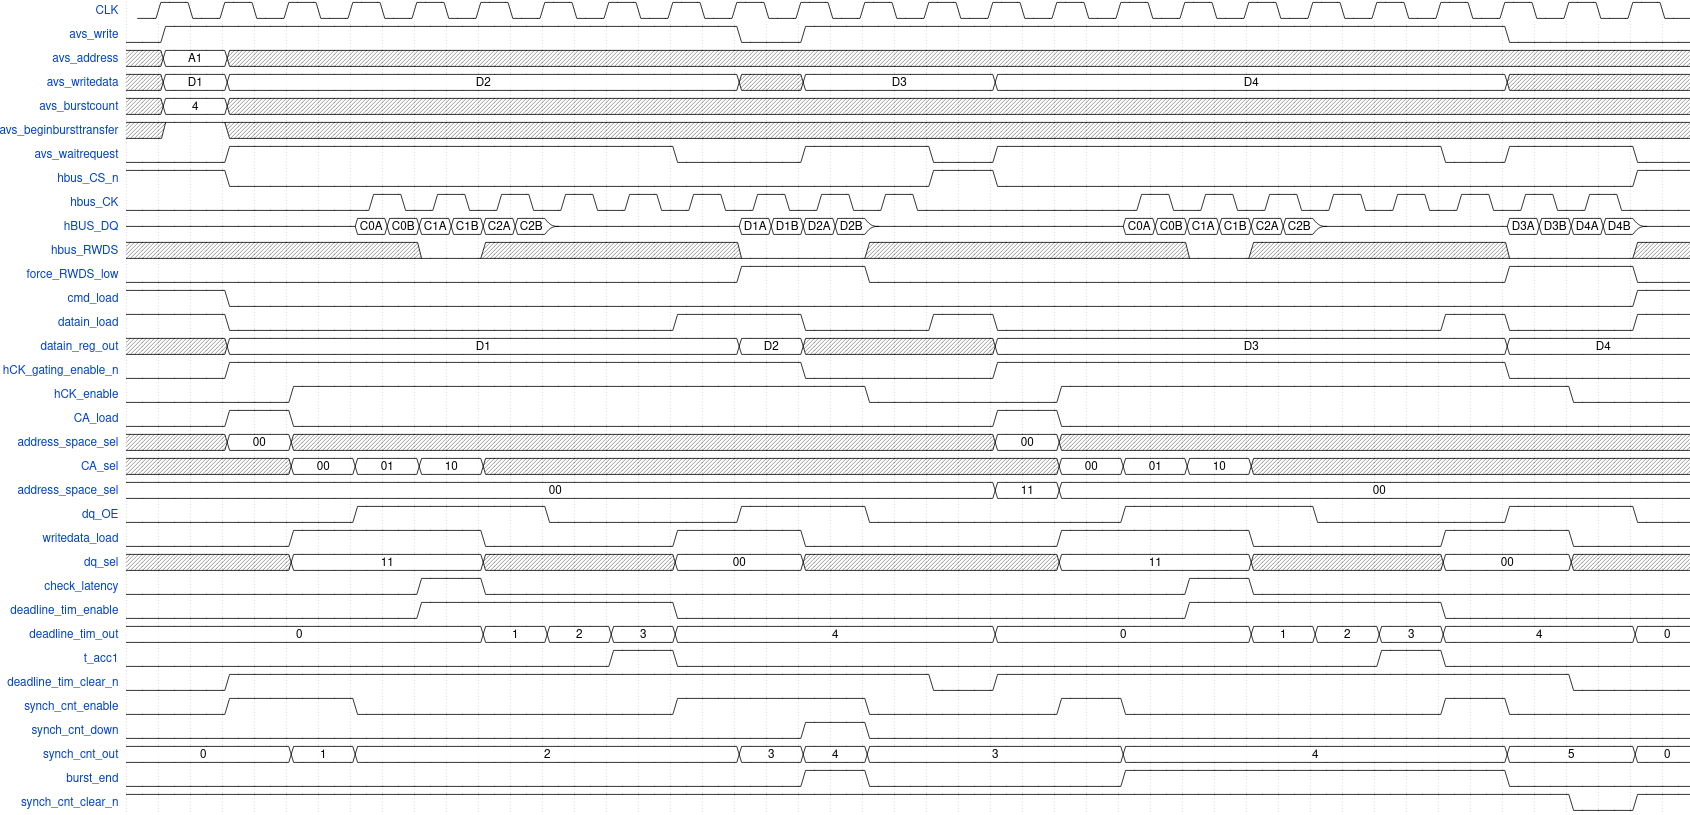
\includegraphics[width=17.5cm]{conv_writeburst_stop.png}
    \caption{\centering Write burst operation with burst interruption.}
    \label{conv_writeburst_stop}
\end{figure}
\vspace{6mm}
\subsection{Memory Timing Constraints} \label{timing_constraints}
\vspace{2mm}
As we can see in figures \ref{hram_read} and \ref{hram_write}, several timing contraints (whose value is listed in figure \ref{hram_timing_param}) must be respected to ensure the correct functioning of the memory:
\vspace{2mm}
\begin{itemize}
    \item \textbf{T\textsubscript{CSHI}} : always ensured by the FSM
    \item \textbf{T\textsubscript{CSS}} : always ensured by the FSM
    \item \textbf{T\textsubscript{RWR}} : always ensured by the FSM
    \item \textbf{T\textsubscript{ACC}} : always ensured by the FSM
    \item \textbf{T\textsubscript{CSH}} : always ensured being null
    \item \textbf{T\textsubscript{DSV}} : always ensured by the FSM
    \item \textbf{T\textsubscript{CKDS}}, \textbf{T\textsubscript{CKD}} : irrelevant, the trace delay is not considered
    \item \textbf{T\textsubscript{DSZ}} (read operation) : irrelevant, only the edges of RWDS are significant
    \item \textbf{T\textsubscript{DSZ}} (write operation) : irrelevant, RWDS is acquired early enough
    \item \textbf{T\textsubscript{DSS}}, \textbf{T\textsubscript{DSH}} : irrelevant, they do not affect the oversampling
    \item \textbf{T\textsubscript{OZ}} : irrelevant, the value of DQ is relevant only in correspondence of the edges of RWDS
    \item \textbf{T\textsubscript{DQLZ}} : irrelevant, the value of DQ is relevant only in correspondence of the edges of RWDS
    \item \textbf{T\textsubscript{CSM}} : it limits the maximum burst lenght
    \item \textbf{T\textsubscript{IS}}, \textbf{T\textsubscript{IH}} : forced during synthesis
\end{itemize}
\vspace{4mm}
Ideally, the \textit{clock shifter} introduces a delay (T\textsubscript{CKSH}) between the internal clock and the HyperRAM clock equal to 90° (5 ns). However, in the real case this delay is characterized by an uncertainty of $\pm$50 ps. Moreover, the \textit{clock controller} introduces an additional delay term (T\textsubscript{CLKCTRL}). Similarly, a certain combinational delay (T\textsubscript{CLKDQ}) is present between the main clock and DQ. All this considered, the actual delay between DQ and the HyperRAM clock (T\textsubscript{IS}) is definitely different from 90°. To ensure the constraint on the minimum value of T\textsubscript{IS} it is necessary to consider the worst case on T\textsubscript{CKSH} and to force a constraint on T\textsubscript{CLKDQ} during the synthesis:
\vspace{4mm}
\begin{center}
    T\textsubscript{IS} = T\textsubscript{CKSH} + T\textsubscript{CLKCTRL} - T\textsubscript{CLKDQ} $\hspace{5mm}$ min\{T\textsubscript{CKSH}\} = 4.95 ns $\hspace{5mm}$ min\{T\textsubscript{CLKCTRL}\} = 0 ns \\
    \vspace{4mm}
    T\textsubscript{IS} $>$ 1 ns $\hspace{5mm} \Rightarrow \hspace{5mm}$  T\textsubscript{CLKDQ} $<$ 3.95 ns
    \vspace{4mm}
\end{center}
The condition T\textsubscript{CLKDQ} $<$ 3.95 ns can be easily satisfied during the synthesis. Actually, this condition has been extended to T\textsubscript{CLKDQ} $<$ 1 ns to have some margin, since the synthesizer does not have any issue to satisfy it. \\ \\
When it comes to the constraint on T\textsubscript{IH}:
\vspace{4mm}
\begin{center}
    10 ns - T\textsubscript{IH} = T\textsubscript{CKSH} + T\textsubscript{CLKCTRL} - T\textsubscript{CLKDQ} $\hspace{5mm}$ max\{T\textsubscript{CKSH}\} = 5.05 ns $\hspace{5mm}$ min\{T\textsubscript{CLKDQ}\} = 0 ns \\
    \vspace{4mm}
    T\textsubscript{IH} $>$ 1 ns $\hspace{5mm} \Rightarrow \hspace{5mm}$  T\textsubscript{CLKCTRL} $<$ 3.95 ns
    \vspace{4mm}
\end{center}
The \textit{clock controller} is a particular IP already available in the Intel catalog. Unfortunately, its documentation does not specify its delay. However, the condition T\textsubscript{CLKCTRL} $<$ 3.95 ns is not that strict, therefore we can assume that it is always satisfied. \\ \\
T\textsubscript{CSM} limits the maximum burst lenght. In the worst case (doubled access time, read operation), a latency of 12 clock periods must be considered between the assertion of \textit{hram\_CS\_n} and the beginning of the burst transfer (as we can see in figure \ref{read_prelimsim_pt1}). Moreover, at the end of the burst trasfer 7 additional clock cycles are required before de-asserting \textit{hram\_CS\_n} (as shown in figure \ref{read_prelimsim_pt2}). As a result:
\vspace{4mm}
\begin{center}
    12 T\textsubscript{CLK} + 7 T\textsubscript{CLK} + N\textsubscript{BURST} T\textsubscript{CLK} $<$ max\{T\textsubscript{CSM}\} = 4 $\mu$s $\hspace{5mm} \Rightarrow \hspace{5mm}$ N\textsubscript{BURST} $<$ 181
    \vspace{4mm}
\end{center}
As we can see, even though the burst lenght is expressed on 11 bits, only 9 bits are actually necessary.

% -------------------------------------------------------------------------------------------------
\chapter{TEST RESULTS} \label{test result}
% -------------------------------------------------------------------------------------------------
\noindent To test the interface converter against a large number of different stimuli it can be inserted in a processor-based system, as represented in figure \ref{test_environment}. However, even if this approach allows to test the \acrshort{DUT} under several different condition, it is possible that some particular operations of our interest are never tested. For instance, the processor may never try to put the memory in DPD mode. For this reason, it was decided to perform different analysis:
\vspace{2mm}
\begin{itemize}
    \item \textbf{Preliminary simulation}: a custom testbench is created to directly drive the interface converter in order to verify its behavior under specific conditions.
    \vspace{1mm}
    \item \textbf{Final simulation}: the interface converter is inserted in the processor-based system (figure \ref{test_environment}) to simulate it against a large number of data.
    \vspace{1mm}
    \item \textbf{Test on VirtLAB}: the processor-based system containing the interface converter is synthesized in the FPGA.
\end{itemize}
\vspace{4mm}
\section{Preliminary Simulation}
\begin{figure}[H]
    \centering
    \captionsetup{width=18cm}
    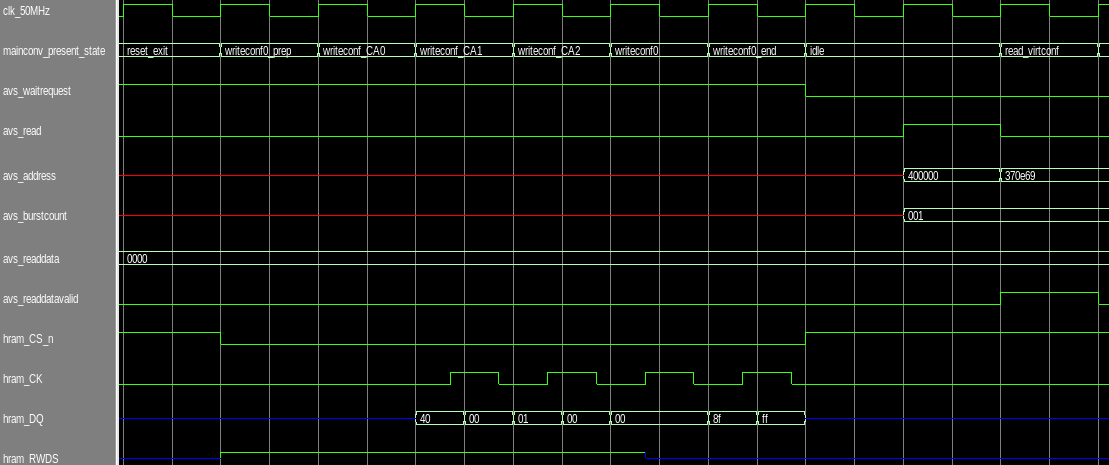
\includegraphics[width=18cm]{writeconf_prelimsim.png}
    \caption{\centering Automatic configuration register update after power-on.}
    \label{writeconf_prelimsim}
\end{figure}
\begin{figure}[H]
    \centering
    \captionsetup{width=18cm}
    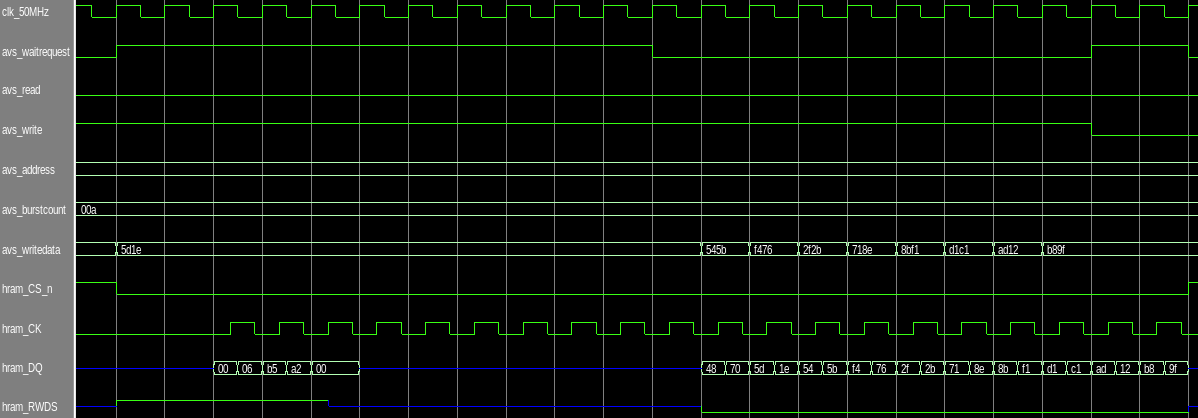
\includegraphics[width=18cm]{write_prelimsim.png}
    \caption{\centering Write operation.}
    \label{write_prelimsim}
\end{figure}
\begin{figure}[H]
    \centering
    \captionsetup{width=18cm}
    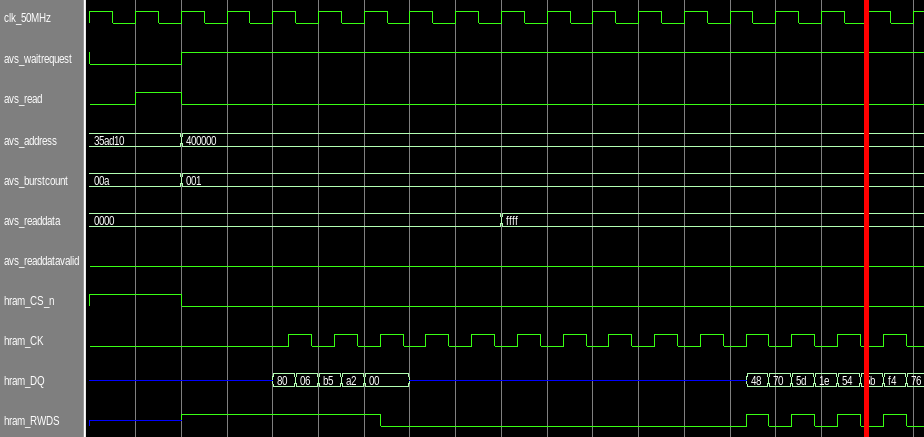
\includegraphics[width=18cm]{read_prelimsim_pt1.png}
    \caption{\centering Read operation - part 1.}
    \label{read_prelimsim_pt1}
\end{figure}
\begin{figure}[H]
    \centering
    \captionsetup{width=18cm}
    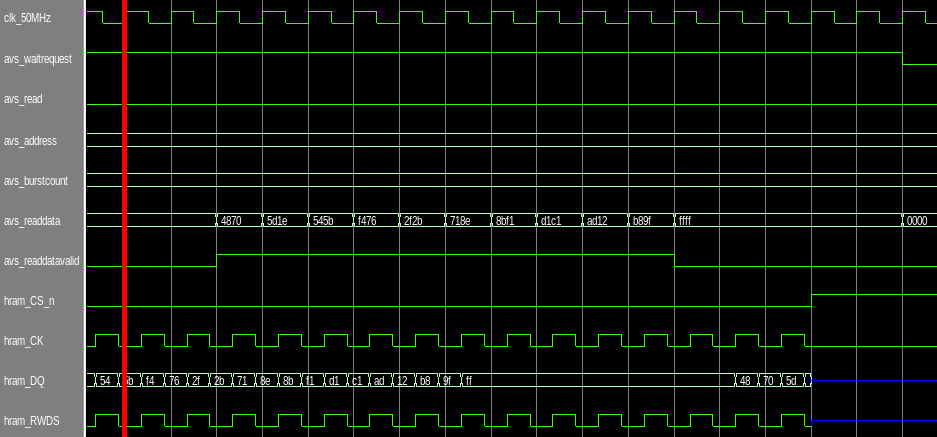
\includegraphics[width=18cm]{read_prelimsim_pt2.png}
    \caption{\centering Read operation - part 2.}
    \label{read_prelimsim_pt2}
\end{figure}
\vspace{4mm}
As we can see in figure \ref{writeconf_prelimsim}, the system automatically initialize CR0 after the power-up as expected (refer to section \ref{CU}). Moreover, a virtual configuration register read operation is succesfully completed. \\ \\
Other than the write operation (figure \ref{write_prelimsim}) and the read configuration (figures \ref{read_prelimsim_pt1} and \ref{read_prelimsim_pt2}), it is important to simulate the behavior of the system in DPD mode. In particular, it must be able to:
\vspace{2mm}
\begin{itemize}
    \item enter the DPD mode when requested (figure \ref{enterDPD_prelimsim})
    \item ignore any operation beside a DPD exit request (figure \ref{DPD_prelimsim})
    \item exit the DPD mode when requested (figures \ref{DPD_prelimsim} and \ref{exitDPD_prelimsim})
    \item automatically update the value of CR0 after exiting the DPD mode (figure \ref{writeconf_postDPD_prelimsim})
\end{itemize}
\vspace{4mm}
\begin{figure}[H]
    \centering
    \captionsetup{width=18cm}
    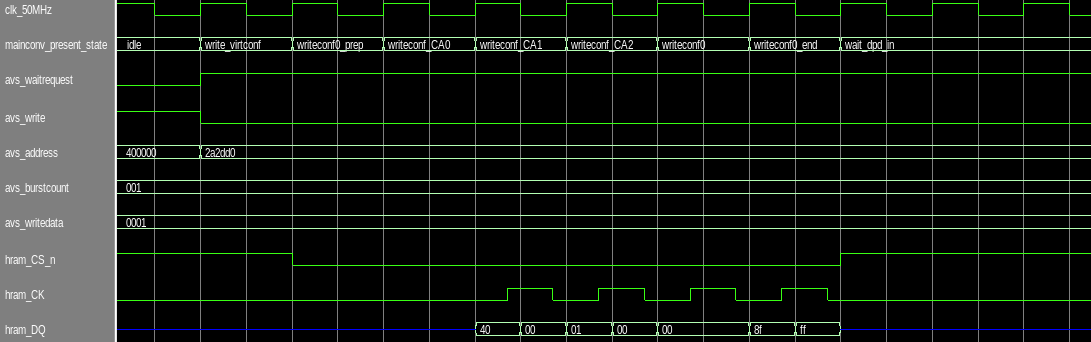
\includegraphics[width=18cm]{enterDPD_prelimsim.png}
    \caption{\centering DPD mode entry request.}
    \label{enterDPD_prelimsim}
\end{figure}
\begin{figure}[H]
    \centering
    \captionsetup{width=18cm}
    \includegraphics[width=18cm]{DPD_prelimsim.png}
    \caption{\centering Ignored read operation and DPD mode exit request.}
    \label{DPD_prelimsim}
\end{figure}
\begin{figure}[H]
    \centering
    \captionsetup{width=18cm}
    \includegraphics[width=18cm]{exitDPD_prelimsim.png}
    \caption{\centering DPD mode exit.}
    \label{exitDPD_prelimsim}
\end{figure}
\begin{figure}[H]
    \centering
    \captionsetup{width=18cm}
    \includegraphics[width=18cm]{writeconf_postDPD_prelimsim.png}
    \caption{\centering Automatic CR0 update after going back to normal mode.}
    \label{writeconf_postDPD_prelimsim}
\end{figure}
\vspace{6mm}
\section{Final Simulation}
\vspace{2mm}
The interface converter is inserted in a processor-based system to simulate it against a large number of data, as we can see in figure \ref{test_environment}. The \textit{Nios II} processor is programmed to read four different signals provided by the \textit{input generator} and to drive four different LEDs according to their value: when a status signal is set, the LED associated with it is turned on and viceversa. The HyperRAM (together with the interface converter) is employed as data memory for the \textit{Nios II} processor.
\vspace{4mm}
\begin{figure}[H]
    \centering
    \captionsetup{width=18cm}
    \includegraphics[width=17cm]{read1_finalsim.png}
    \caption{\centering One of the many read operations driven by the processor - part 1.}
    \label{read1_finalsim}
\end{figure}
\begin{figure}[H]
    \centering
    \captionsetup{width=18cm}
    \includegraphics[width=17cm]{read2_finalsim.png}
    \caption{\centering One of the many read operations driven by the processor - part 2.}
    \label{read2_finalsim}
\end{figure}
\begin{figure}[H]
    \centering
    \captionsetup{width=18cm}
    \includegraphics[width=18cm]{write_finalsim.png}
    \caption{\centering One of the many write operations driven by the processor.}
    \label{write_finalsim}
\end{figure}
\begin{figure}[H]
    \centering
    \captionsetup{width=16cm}
    \includegraphics[width=18cm]{timing_finalsim.png}
    \caption{\centering Processor-based system behavior.}
    \label{timing_finalsim}
\end{figure}
\vspace{4mm}
\noindent At first, the processor-based system must wait for the memory to power-up, therefore it cannot process the input values, as we can see in figure \ref{timing_finalsim}. Indeed, during this initial time interval the LEDs are constantly turned off regardless of the value of the inputs. When the memory is powered-up, the processor drives the LEDs according to the input values as expected.
\vspace{6mm}
\section{Test on VirtLAB}
% -------------------------------------------------------------------------------------------------
\chapter{FUTURE EXTENSIONS}
\noindent The designed system is capable of correctly interface the HyperRAM with the Intel Avalon bus. However, it is still possible to work on some details to improve its performance. In particular:
\vspace{2mm}
\begin{itemize}
    \item As described in section \ref{Readdata Converter}, the working frequency of the memory has been reduced to 50 MHz due to the limitations related to the oversampling. However, all the other components of the system are able to work at 100 MHz. Indeed, exploiting a controlled combinational delay (instead of the oversampling) to implement the \textit{readdata converter} would allow to push the working frequency up to 100 MHz.
    \item On the Avalon side, the burst lenght is characterized by a parallelism of 11 bits. However, the burst lenght value cannot be higher than 181, therefore only 9 bits are actually useful, as described in section \ref{timing_constraints}. For this reason, the counter and the comparator inside the \textit{synchronizer} (\textit{burstlen\_counter} and \textit{burstlen\_cmp} referring to figure \ref{synchronizer_EU}) can be implemented with a reduced parallelism, saving power and resources.
    \item The virtual configuration register allows to dynamically modify only two parameters of the HyperRAM (working mode and memory access latency). However, the design can be easily modified to allow the host to access also other parameters.
\end{itemize}

% -------------------------------------------------------------------------------------------------

% \cite{cit_tag}
\begin{thebibliography}{1}
    \bibitem{virtlab} Massimo Ruo Roch, Maurizio Martina, \emph{VirtLAB: a Low-Cost Platform for Electronic Lab experiments}, Sensors
\end{thebibliography}


\end{document}
